\begin{chapterenv}

\chapter{Modern RL Algorithms: GRPO, RLOO, KTO \& More}

\section{The Algorithm Landscape}

Chapters 6 and 7 introduced the two workhorses of LLM alignment: PPO (the classical RL approach with a reward model, value function, and clipped policy updates) and DPO (the elegant shortcut that trains directly on preference pairs). Together they cover a wide range of practical needs, but neither is the final word. Since 2023, researchers have introduced a family of alternatives, each designed to solve a specific limitation.

Some of these algorithms eliminate the value function that makes PPO expensive. Others work with cheaper forms of feedback than paired comparisons. Still others merge supervised learning and preference optimization into a single training stage. This chapter surveys the most important ones: GRPO, RLOO, KTO, IPO, and ORPO.

Before diving into individual algorithms, it helps to see the full landscape at a glance.

\begin{figure}[!h]
\centering
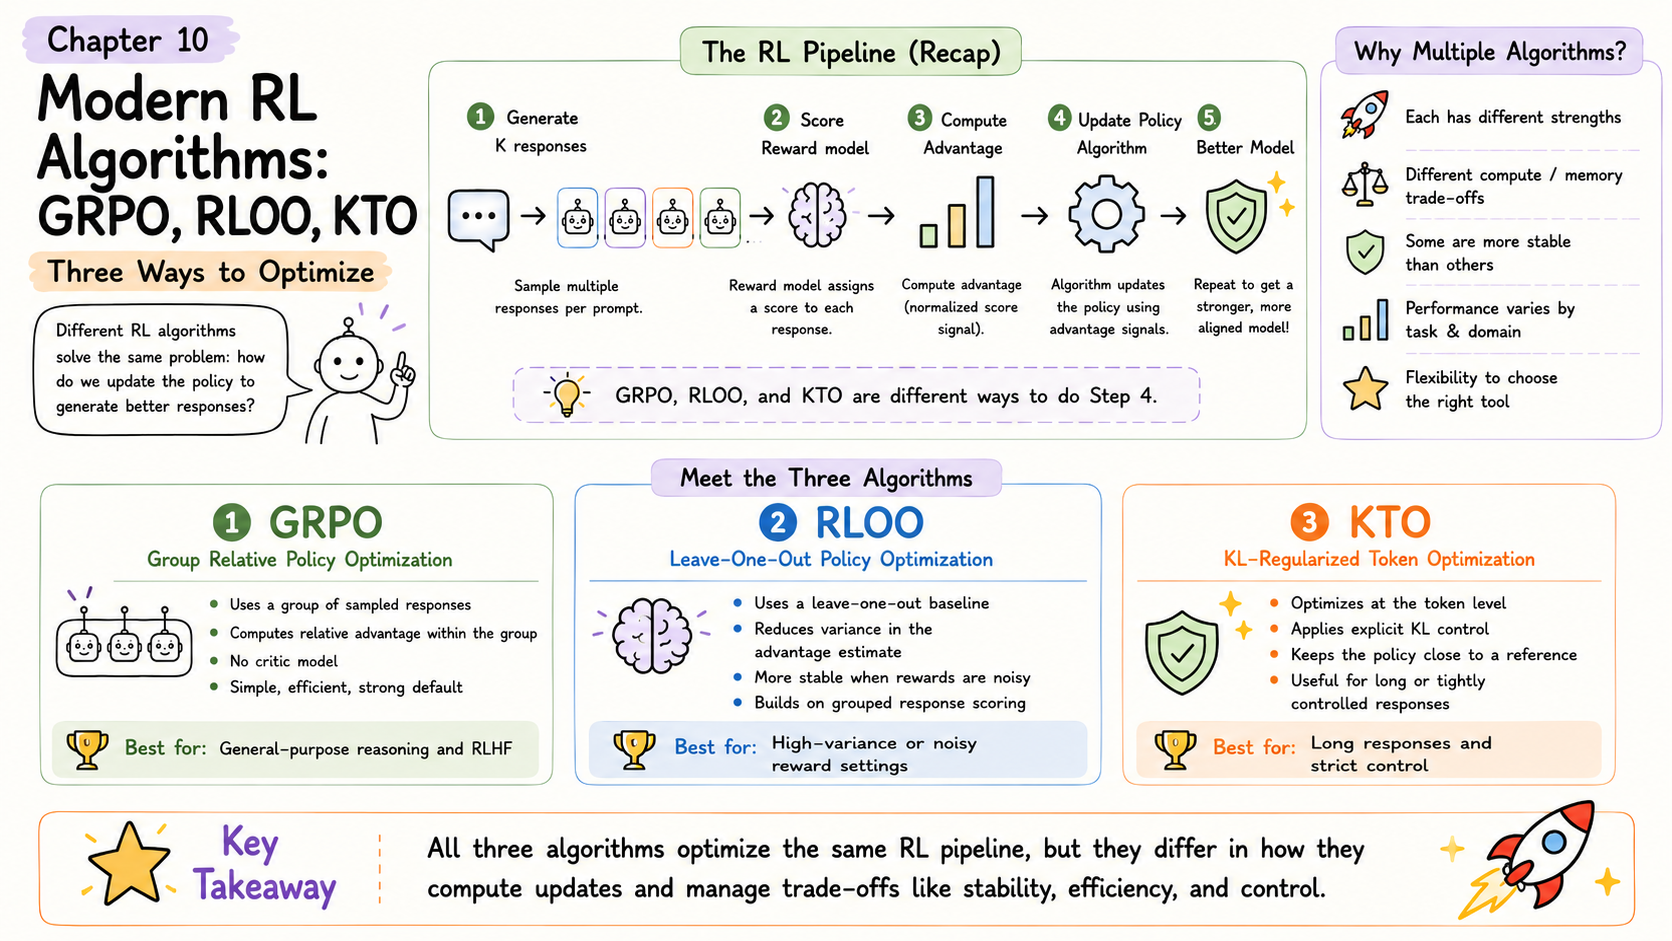
\includegraphics[width=0.88\textwidth]{images/ch10_fig01_grpo_rloo_kto_intro.png}
\caption{Modern RL algorithms at a glance -- GRPO, RLOO, and KTO: three ways to update the policy without a critic.}
\label{fig:ch10:grpo_rloo_kto_intro}
\end{figure}

\begin{center}
\begin{tabular}{p{0.10\textwidth}p{0.22\textwidth}p{0.17\textwidth}p{0.12\textwidth}p{0.22\textwidth}}
\toprule
\textbf{Algorithm} & \textbf{Key Innovation} & \textbf{Data Required} & \textbf{Models in Memory} & \textbf{Best For} \\
\midrule
PPO & Clipped policy gradient with learned critic & Reward model scores & 4 (policy, ref, RM, critic) & Maximum performance, abundant compute \\
DPO & Implicit reward from policy ratios & Paired preferences & 2 (policy, ref) & Simplicity with paired data \\
GRPO & Group average as baseline & Reward scores + group sampling & 2 (policy, ref) & Large-scale training, verifiable tasks \\
RLOO & Leave-one-out baselines & Reward scores + group sampling & 2 (policy, ref) & Efficient RL without critic \\
KTO & Works with unpaired feedback & Binary good/bad labels & 2 (policy, ref) & Cheap data, no comparisons needed \\
IPO & Squared loss with explicit gap target & Paired preferences & 2 (policy, ref) & Stability, preventing reward hacking \\
ORPO & Merges SFT and preference learning & Paired preferences + demos & 1 (policy only) & Maximum efficiency, tight compute \\
\bottomrule
\end{tabular}
\end{center}

We begin with REINFORCE, the simplest policy gradient algorithm and the mathematical foundation on which both GRPO and RLOO are built. Understanding it first makes the innovations in those algorithms much clearer.

\section{REINFORCE: The Foundation}

Every policy gradient algorithm in this chapter descends from a single idea: generate a response, score it, and adjust the policy to make high-scoring responses more likely. REINFORCE is the simplest version of this idea.

\begin{infobox}
\textbf{The REINFORCE Gradient}

$$\nabla J(\theta) = \mathbb{E}_{y \sim \pi_\theta}\!\left[r(y) \cdot \nabla \log \pi_\theta(y|x)\right]$$

\textbf{In plain English:} Sample a response $y$ from the current policy. Get its reward $r(y)$. If the reward is high, adjust the policy to make $y$ more likely. If the reward is low, make $y$ less likely. The magnitude of the adjustment is proportional to the reward.
\end{infobox}

The problem with vanilla REINFORCE is \textit{variance}. Suppose all your rewards happen to be positive (say, between 3 and 8). Then every response gets pushed to be more likely, just by different amounts. The model learns slowly because the gradient signal is dominated by the absolute reward level rather than relative quality.

\textbf{Baselines reduce variance.} Subtracting a baseline $b$ from the reward fixes this:

$$\nabla J(\theta) = \mathbb{E}_{y \sim \pi_\theta}\!\left[(r(y) - b) \cdot \nabla \log \pi_\theta(y|x)\right]$$

Now responses with reward above the baseline get positive updates (``do more of this'') and responses below the baseline get negative updates (``do less of this''). The signal becomes about relative quality, not absolute scores. Crucially, subtracting any constant baseline does not change the expected gradient--it only reduces its variance.

\textbf{The question every algorithm answers differently is: what should $b$ be?}

\begin{center}
\begin{tabular}{lp{0.65\textwidth}}
\toprule
\textbf{Algorithm} & \textbf{Baseline choice} \\
\midrule
REINFORCE & A fixed constant (e.g., running average of all rewards) \\
PPO & A learned value function $V_\psi(x)$ that predicts expected reward for each prompt--accurate but expensive (requires a separate neural network) \\
GRPO & The average reward within a group of responses to the \textit{same prompt}--adaptive and free \\
RLOO & The average reward of all \textit{other} responses in the group (leave-one-out)--even lower variance than GRPO \\
\bottomrule
\end{tabular}
\end{center}

REINFORCE itself is rarely used in production LLM training because its variance is too high for stable learning at scale. But understanding it makes GRPO and RLOO immediately intuitive: they are REINFORCE with clever, cheap baselines.

\section{GRPO: Group Relative Policy Optimization}

GRPO was introduced by DeepSeek and used to train DeepSeek-R1. It replaces PPO's learned value function (the critic) with a much simpler idea: for each prompt, generate a \textit{group} of responses, score them all, and use the group's average score as the baseline. Responses that score above the group average are reinforced; responses that score below are discouraged.

This is the same principle as REINFORCE with a baseline, but the baseline adapts automatically to each prompt's difficulty. A hard math problem where the model gets 1 out of 4 correct will have a low group average, so the single correct response gets a strong positive signal. An easy problem where the model gets 3 out of 4 correct will have a high group average, so only the best responses are reinforced strongly. No learned critic needed.

\begin{infobox}
\textbf{GRPO Objective}

$$\mathcal{L}_{\text{GRPO}} = -\mathbb{E}_{x,\{y_i\}_{i=1}^G}\!\left[\frac{1}{G}\sum_{i=1}^{G}\left(\hat{A}_i\right) \cdot \min\!\left(\rho_i \hat{A}_i,\; \text{clip}(\rho_i, 1{-}\epsilon, 1{+}\epsilon)\,\hat{A}_i\right)\right] + \beta \cdot \text{KL}(\pi_\theta \,\|\, \pi_{\text{ref}})$$

\textbf{Core idea:} Generate a group of $G$ responses per prompt, use the group's own statistics as the baseline, and apply PPO-style clipping to stabilize updates.
\end{infobox}

\textbf{Breaking apart the components:} $G$ is the group size (typically 4--8 responses per prompt). $\hat{A}_i = \frac{r(x, y_i) - \bar{r}_G}{\sigma_G}$ is the normalized advantage--the reward for response $i$ minus the group mean, divided by the group standard deviation. $\rho_i = \frac{\pi_\theta(y_i|x)}{\pi_{\text{old}}(y_i|x)}$ is the importance sampling ratio, clipped in the same way as PPO. $\bar{r}_G = \frac{1}{G}\sum_{j=1}^{G}r(x, y_j)$ is the group mean reward, and $\beta \cdot \text{KL}$ penalizes drift from the reference model.

That is the full production version. The core insight is simpler: $\hat{A}_i$ replaces PPO's learned value function. Instead of training a separate neural network to predict ``how good should a response to this prompt be?'', GRPO just asks ``how good is this response compared to the other responses in its group?''

\subsection{GRPO Walkthrough}

\textbf{Problem:} ``What is $\sqrt{144} + 12 \times 3$?'' \quad \textbf{Correct answer:} 48

\textbf{Step 1: Generate a group of 4 attempts.}

\begin{center}
\begin{tabular}{p{0.10\textwidth}p{0.45\textwidth}p{0.18\textwidth}p{0.10\textwidth}}
\toprule
\textbf{Attempt} & \textbf{Model Output} & \textbf{Answer} & \textbf{Reward} \\
\midrule
1 & ``$12 + 36 = 48$'' & 48 (correct) & +1 \\
2 & ``$\sqrt{144} = 12$, then $12 + 12 \times 3$\ldots'' & 48 (correct) & +1 \\
3 & ``$\sqrt{144} = 14$, $14 + 36 = 50$'' & 50 (wrong) & 0 \\
4 & ``$144 + 36 = 180$'' & 180 (wrong) & 0 \\
\bottomrule
\end{tabular}
\end{center}

\textbf{Step 2: Compute group statistics.}

$$\bar{r}_G = \frac{1 + 1 + 0 + 0}{4} = 0.5 \qquad \sigma_G = 0.5$$

\textbf{Step 3: Compute normalized advantages.}

\begin{center}
\begin{tabular}{ccccc}
\toprule
\textbf{Attempt} & \textbf{Reward} & \textbf{$r - \bar{r}_G$} & \textbf{$\hat{A} = (r - \bar{r}_G)/\sigma_G$} & \textbf{Update Direction} \\
\midrule
1 & +1 & +0.5 & +1.0 & Increase probability \\
2 & +1 & +0.5 & +1.0 & Increase probability \\
3 & 0 & $-0.5$ & $-1.0$ & Decrease probability \\
4 & 0 & $-0.5$ & $-1.0$ & Decrease probability \\
\bottomrule
\end{tabular}
\end{center}

\textbf{Step 4: Update the policy.} Attempts 1 and 2 (correct, with step-by-step reasoning) become more likely. Attempts 3 and 4 (errors from skipping steps or miscalculating) become less likely. Over many problems and many groups, the model discovers that detailed reasoning leads to better rewards.

\begin{tipbox}
\textbf{Why normalization matters.} Dividing by $\sigma_G$ ensures that the advantage magnitude is consistent across prompts. A prompt where all 4 responses are correct (rewards: 1, 1, 1, 1) has $\sigma_G = 0$, so no gradient is produced--the model has nothing to learn from that prompt. A prompt where responses vary widely produces large advantages and strong learning signals. This automatic calibration is one of GRPO's key practical benefits.
\end{tipbox}

\subsection{GRPO vs PPO: What Changes}

\begin{center}
\begin{tabular}{p{0.25\textwidth}p{0.30\textwidth}p{0.30\textwidth}}
\toprule
\textbf{Component} & \textbf{PPO} & \textbf{GRPO} \\
\midrule
Baseline / advantage & Learned value function $V_\psi(x)$ & Group mean $\bar{r}_G$ (no learned parameters) \\
Extra model & Critic network (trainable) & None \\
Samples per prompt & Typically 1 & $G$ samples (4--8 typical) \\
Clipping & Yes ($\epsilon = 0.2$) & Yes (same mechanism) \\
KL regularization & KL penalty in reward & Explicit KL term in loss \\
Memory & 4 models & 2 models \\
\bottomrule
\end{tabular}
\end{center}

\textbf{The trade-off:} GRPO saves memory (no critic) and implementation complexity, but requires generating multiple responses per prompt, which increases inference cost. For tasks with cheap, verifiable rewards (math, code execution, factual questions), this trade-off is strongly favorable. For tasks where scoring is expensive (human evaluation), the extra generation cost can be significant.

\begin{infobox}
\textbf{Practical considerations for GRPO}

\textbf{Group size.} $G = 4$ is the minimum for meaningful statistics. $G = 8$ gives more stable baselines. Beyond $G = 16$, the marginal improvement in variance reduction is small relative to the extra generation cost.

\textbf{Reward design.} GRPO works best with binary or near-binary rewards (correct/incorrect) because the group statistics are most informative when there is variance within the group. If every response gets reward 0.7--0.8, the advantages are tiny and learning is slow.

\textbf{KL penalty.} The $\beta$ term serves the same role as in RLHF (Chapter 6): preventing the policy from drifting too far from the reference. Typical values are $\beta = 0.01$ to $0.05$. Without it, the model can collapse to always producing the same response format.

\textbf{When to choose GRPO:} Tasks with verifiable rewards (math, code, factual QA), large-scale training where critic memory is a bottleneck, and settings where you want PPO-like online exploration without PPO's complexity. Chapter 12 covers how DeepSeek applied GRPO at scale to produce reasoning capabilities.
\end{infobox}

\section{RLOO: REINFORCE Leave-One-Out}



RLOO refines the baseline idea one step further. Like GRPO, it generates a group of responses per prompt. But instead of comparing each response against the group average (which includes that response), it compares each response against the average of the \textit{other} responses in the group. This small change produces meaningfully lower variance.

\begin{infobox}
\textbf{RLOO Baseline}

For a group of $N$ responses $\{y_1, \ldots, y_N\}$ to prompt $x$, the leave-one-out baseline for response $i$ is:

$$b_{-i} = \frac{1}{N-1}\sum_{j \neq i} r(x, y_j)$$

The gradient for response $i$ becomes:

$$\nabla \mathcal{L}_i = (r(x, y_i) - b_{-i}) \cdot \nabla \log \pi_\theta(y_i | x)$$

\textbf{Key insight:} Each response is compared against a baseline that does not include its own reward. This prevents a high-reward response from inflating its own baseline and thereby reducing its own learning signal.
\end{infobox}

\subsection{RLOO Walkthrough}

\textbf{Prompt:} ``Write a poem about spring''

\begin{center}
\begin{tabular}{clc}
\toprule
\textbf{\#} & \textbf{Response} & \textbf{Reward} \\
\midrule
1 & ``Spring is nice\ldots'' (mediocre) & 3 \\
2 & ``Blossoms dance in gentle breeze\ldots'' (good) & 8 \\
3 & ``Spring spring spring\ldots'' (bad) & 1 \\
4 & ``Flowers bloom as winter ends\ldots'' (okay) & 5 \\
\bottomrule
\end{tabular}
\end{center}

\textbf{Standard REINFORCE baseline} (group average including all responses):

$$b = \frac{3 + 8 + 1 + 5}{4} = 4.25$$

Advantages: $-1.25$, $+3.75$, $-3.25$, $+0.75$

\textbf{RLOO baselines} (leave-one-out):

\begin{center}
\begin{tabular}{ccccl}
\toprule
\textbf{Response} & \textbf{Reward} & \textbf{Leave-one-out baseline} & \textbf{Advantage} & \textbf{vs.\ standard} \\
\midrule
1 & 3 & $(8+1+5)/3 = 4.67$ & $-1.67$ & Stronger decrease \\
2 & 8 & $(3+1+5)/3 = 3.00$ & $+5.00$ & Stronger increase \\
3 & 1 & $(3+8+5)/3 = 5.33$ & $-4.33$ & Stronger decrease \\
4 & 5 & $(3+8+1)/3 = 4.00$ & $+1.00$ & Stronger increase \\
\bottomrule
\end{tabular}
\end{center}

The RLOO advantages have \textit{larger magnitude} than the standard ones. Response 2 (the best) gets an advantage of $+5.0$ instead of $+3.75$, because its own high score no longer inflates the baseline. Response 3 (the worst) gets $-4.33$ instead of $-3.25$, because its own low score no longer deflates the baseline. The result is sharper learning signals and faster convergence.

\begin{tipbox}
\textbf{RLOO vs GRPO.} Both eliminate the critic and use group-based baselines. The differences are subtle: GRPO normalizes advantages by the group standard deviation and uses PPO-style clipping; RLOO uses leave-one-out baselines without normalization and applies the gradient more directly. In practice, both produce comparable results. RLOO is slightly simpler to implement; GRPO is more widely used because of its association with DeepSeek. RLOO works well with as few as $N = 2$ samples per prompt, while GRPO typically needs $G \geq 4$ for stable statistics.
\end{tipbox}

\section{KTO: Kahneman-Tversky Optimization}

All the methods discussed so far--PPO, DPO, GRPO, RLOO, and the algorithms in Chapter 8--require either paired preferences (``Response A is better than Response B'') or a reward model that produces numerical scores. KTO eliminates both requirements. It works with simple binary feedback: each response is labeled independently as ``good'' or ``bad,'' with no comparison to any other response.

This matters because binary labels are dramatically cheaper to collect. Paired comparisons require showing an annotator two responses to the same prompt and asking which is better. Binary labels only require a single judgment: ``Is this response acceptable?'' This halves annotation cost and is the natural format of much real-world feedback: upvotes, downvotes, thumbs up, star ratings, user retention signals.

\begin{infobox}
\textbf{KTO Loss Function}

For a desirable (good) response $y^+$:

$$\mathcal{L}_{\text{KTO}}^{+} = 1 - \sigma\!\left(\beta \log \frac{\pi_\theta(y^+|x)}{\pi_{\text{ref}}(y^+|x)} - \mathbb{E}_{y \sim \pi_{\text{ref}}}\!\left[\beta \log \frac{\pi_\theta(y|x)}{\pi_{\text{ref}}(y|x)}\right]\right)$$

For an undesirable (bad) response $y^-$:

$$\mathcal{L}_{\text{KTO}}^{-} = \sigma\!\left(\beta \log \frac{\pi_\theta(y^-|x)}{\pi_{\text{ref}}(y^-|x)} - \mathbb{E}_{y \sim \pi_{\text{ref}}}\!\left[\beta \log \frac{\pi_\theta(y|x)}{\pi_{\text{ref}}(y|x)}\right]\right)$$

Total loss: $\mathcal{L}_{\text{KTO}} = \mathbb{E}[\mathcal{L}_{\text{KTO}}^{+}] + \mathbb{E}[\mathcal{L}_{\text{KTO}}^{-}]$

\textbf{In plain English:} For good responses, increase their probability relative to a reference baseline. For bad responses, decrease their probability. The reference expectation term provides implicit comparison--even without paired data.
\end{infobox}

\textbf{The name explained.} KTO is based on Kahneman and Tversky's prospect theory from behavioral economics: humans evaluate outcomes relative to a reference point, not in absolute terms. A salary of \$100K feels great if your reference is \$70K, but disappointing if your reference is \$130K. KTO applies the same principle: the quality of a response is judged relative to what the reference model would typically produce, not by absolute scoring.

\textbf{The reference expectation term} $\mathbb{E}_{y \sim \pi_{\text{ref}}}[\beta \log \frac{\pi_\theta(y|x)}{\pi_{\text{ref}}(y|x)}]$ deserves attention. It measures how much the policy has shifted on average from the reference model's distribution. This term appears in both the good and bad losses, acting as a moving baseline that calibrates the learning signal. Without it, the model might simply increase the probability of everything (good and bad alike) if most examples are labeled good.

\begin{tipbox}
\textbf{When to use KTO}

\textbf{Good fit:} You have upvote/downvote data (Reddit, Stack Overflow style), star ratings that can be binarized, implicit signals (user copied response = good, user regenerated = bad), or a limited annotation budget where paired comparisons are too expensive.

\textbf{Not ideal when:} You already have high-quality paired preferences (DPO will use them more efficiently), you need fine-grained ranking (KTO only distinguishes good from bad, not degrees of quality), or peak performance matters more than data efficiency (KTO slightly underperforms DPO/PPO with abundant paired data).

\textbf{Practical tip:} Use KTO for initial training with cheap binary data, then refine with DPO on a smaller set of high-quality paired preferences. This two-stage approach gets most of the benefit of both methods.
\end{tipbox}

\section{IPO: Identity Preference Optimization}

IPO addresses a specific failure mode of DPO: overfitting to the preference data in a way that produces degenerate behavior. Recall from Chapter 7 that DPO's loss function uses a log-sigmoid that pushes the implicit reward gap between winner and loser as large as possible. In theory, this is fine. In practice, the model can exploit this by learning superficial patterns--such as ``longer responses are usually preferred''--and amplifying them to extreme levels.

IPO replaces DPO's log-sigmoid loss with a squared loss that has an explicit target gap. Instead of ``make the winner as much better as possible,'' IPO says ``make the winner better by exactly $1/\beta$.''

\begin{infobox}
\textbf{IPO Loss Function}

$$\mathcal{L}_{\text{IPO}} = \mathbb{E}\!\left[\left(\log \frac{\pi_\theta(y_w|x)}{\pi_{\text{ref}}(y_w|x)} - \log \frac{\pi_\theta(y_l|x)}{\pi_{\text{ref}}(y_l|x)} - \frac{1}{\beta}\right)^{\!2}\right]$$

\textbf{Compare to DPO:}

$$\mathcal{L}_{\text{DPO}} = -\mathbb{E}\!\left[\log \sigma\!\left(\beta \log \frac{\pi_\theta(y_w|x)}{\pi_{\text{ref}}(y_w|x)} - \beta \log \frac{\pi_\theta(y_l|x)}{\pi_{\text{ref}}(y_l|x)}\right)\right]$$

\textbf{The key difference:} DPO uses log-sigmoid (unbounded optimization--push the gap as large as possible). IPO uses squared error with a target gap of $1/\beta$ (bounded optimization--stop once the gap is right).
\end{infobox}

\textbf{Why the target gap helps.} Think of a sports analogy. DPO is like a coach who says ``win by as much as possible''--the team runs up the score, which wastes energy and can lead to reckless play. IPO is like a coach who says ``win by exactly 10 points''--the team plays efficiently and stops over-optimizing once the margin is achieved. The explicit gap $1/\beta$ prevents the model from over-fitting to easy examples or amplifying spurious correlations in the preference data.

\begin{tipbox}
\textbf{When to choose IPO over DPO}

\textbf{Choose IPO when:} You have observed reward hacking or length exploitation with DPO, training stability matters more than peak performance, or your preference data is noisy (IPO's bounded loss is less sensitive to mislabeled pairs).

\textbf{Stick with DPO when:} Your preference data is clean and high-quality, you want maximum performance and are willing to tune carefully, or you plan to use Online DPO (Chapter 8) which mitigates many of DPO's overfitting issues through fresh data.

\textbf{The trade-off:} IPO sacrifices some peak performance for more predictable, stable training. In benchmarks, IPO typically achieves 95--98\% of DPO's performance with significantly fewer training instabilities.
\end{tipbox}

\section{ORPO: Odds Ratio Preference Optimization}

Every method we have covered so far assumes a two-stage training pipeline: first SFT to teach the model basic instruction following, then a separate preference optimization stage (DPO, PPO, KTO, etc.) to align the model's outputs with human preferences. ORPO eliminates this separation by combining both objectives into a single loss function.

\begin{infobox}
\textbf{ORPO Loss Function}

$$\mathcal{L}_{\text{ORPO}} = \underbrace{-\mathbb{E}\!\left[\log \pi_\theta(y_w|x)\right]}_{\text{SFT term: learn from good responses}} + \;\lambda \cdot \underbrace{\left(-\mathbb{E}\!\left[\log \sigma\!\left(\log \frac{\text{odds}(y_w)}{\text{odds}(y_l)}\right)\right]\right)}_{\text{Preference term: prefer winners over losers}}$$

Where $\text{odds}(y) = \frac{\pi_\theta(y|x)}{1 - \pi_\theta(y|x)}$ and $\lambda$ controls the relative weight (typically 0.1 to 1.0).

\textbf{In plain English:} The SFT term teaches the model to produce good responses. The preference term teaches it to produce good responses \textit{more than} bad ones. Both happen simultaneously in every training step.
\end{infobox}

\textbf{Why odds ratios?} The standard DPO loss compares log probabilities between the policy and reference model. ORPO instead compares the \textit{odds} of the winner and loser under the current policy alone. The odds ratio measures how much more likely the model is to produce the winner than the loser, accounting for the fact that both probabilities must sum with everything else the model can generate. This formulation does not require a reference model at all, which means ORPO needs only one model in memory--the lowest of any method in this chapter.

\textbf{No reference model.} This is ORPO's most distinctive feature. DPO, KTO, and IPO all require keeping a frozen copy of the SFT model as $\pi_{\text{ref}}$. ORPO's odds ratio formulation makes the reference unnecessary because the SFT component of the loss already prevents the policy from drifting into degenerate territory. This saves significant memory, especially for large models.

\begin{tipbox}
\textbf{When to use ORPO}

\textbf{Great choice when:} You have both instruction-following demonstrations and paired preferences for the same data, compute budget is tight (one training run instead of two, one model instead of two), or you are training smaller models where fast iteration matters.

\textbf{Not ideal when:} You need to separately tune SFT and preference learning (different data, different hyperparameters), you have very different data sources for demonstrations vs.\ preferences, or you need state-of-the-art performance (ORPO typically achieves 95--98\% of PPO's quality in roughly half the training time).

\textbf{Practical note:} The weight $\lambda$ between SFT and preference terms requires tuning. Too small ($\lambda < 0.1$) and the model learns to follow instructions but ignores preference quality. Too large ($\lambda > 1.0$) and the model optimizes preferences at the cost of basic fluency. Start with $\lambda = 0.1$ and increase if preference alignment is insufficient.
\end{tipbox}

\section{Choosing the Right Algorithm}

With seven algorithms now in your toolkit, choosing the right one requires matching your constraints to each method's strengths. The decision depends on three factors: what data you have, what compute you can afford, and what matters most for your task.

\begin{infobox}
\textbf{Decision Factor 1: What data do you have?}

\textbf{Paired preferences} (``A is better than B''): DPO, IPO, or ORPO. These methods directly optimize on comparison data. DPO is the default; IPO if you need stability; ORPO if you also want SFT in one stage.

\textbf{Binary labels} (``good'' or ``bad''): KTO. It is the only method in this chapter designed for unpaired feedback. If your data comes from upvotes/downvotes, user retention signals, or simple quality labels, KTO is the natural choice.

\textbf{Reward model or verifier scores}: GRPO or RLOO. These methods generate multiple responses per prompt and use the scores to compute advantages. They require either a trained reward model (Chapter 9) or a deterministic verifier (e.g., code execution, math checker).
\end{infobox}

\begin{infobox}
\textbf{Decision Factor 2: What is your compute budget?}

\textbf{High} (multi-GPU cluster, large-scale training): PPO or GRPO. PPO gives the highest performance ceiling with abundant compute. GRPO is the go-to for verifiable tasks at scale (it powered DeepSeek-R1).

\textbf{Medium} (single GPU or small cluster): DPO, IPO, or RLOO. DPO and IPO need only two models and train like supervised learning. RLOO needs two models plus multi-sample generation but avoids a learned critic.

\textbf{Low} (consumer GPU, tight memory): ORPO (one model, one training stage) or KTO (two models, but simple binary data pipeline).
\end{infobox}

\begin{infobox}
\textbf{Decision Factor 3: What is your priority?}

\textbf{Peak performance:} PPO (with enough compute) or GRPO (for verifiable tasks). These online methods explore beyond the training data, which DPO cannot.

\textbf{Training stability:} IPO (explicit gap prevents overfitting) or GRPO (normalized advantages, automatic difficulty calibration).

\textbf{Data efficiency:} KTO (needs only binary labels, halving annotation cost) or ORPO (combines SFT and alignment, fewer total training steps).

\textbf{Implementation simplicity:} DPO (most widely documented, best library support in TRL, closest to standard supervised training).
\end{infobox}

\begin{tipbox}
\textbf{The practitioner's starting point.}

If you are unsure, start with DPO. It has the best documentation, the most library support (TRL's \texttt{DPOTrainer}), and produces strong results with minimal tuning. Then move to a specialized algorithm if you hit a specific problem:

DPO overfitting or reward hacking $\to$ try IPO.

No paired preference data $\to$ try KTO.

Need exploration beyond offline data $\to$ try GRPO or Online DPO (Chapter 8).

Want to skip separate SFT stage $\to$ try ORPO.

Need maximum performance with abundant compute $\to$ try PPO (Chapter 6).

Chapter 12 will show how GRPO was applied at scale in the DeepSeek recipe to produce reasoning capabilities, and Chapter 17 will combine multiple algorithms into end-to-end training recipes for chatbots, reasoners, and agents.
\end{tipbox}


The companion code for this chapter is at \texttt{github.com/arunpshankar/packt-final} -- swap \texttt{github.com} for \texttt{githubtocolab.com} to open it directly in Colab.

\end{chapterenv}